% !Mode:: "TeX:UTF-8"

\chapter[并行计算圆周率]{并行计算圆周率$\pi$}
\section{圆周率算法介绍}
    圆周率,一般用$\pi$来表示,其定义为圆形之周长与直径之比,它是精确计算圆周长,圆面积,球体积等几何形状的关键
。
    
    常见的计算圆周率方法为马青公式,马青公式的反正切公式,拉马努公式,高斯-勒让德公式等等,本文着重讨论和研究使
用微积分的方式计算$\pi$,见式$1-1$
   $$ \int_0^1 \frac{4\,dx}{1+x^2} =  \int_0^\frac{\pi}{4}  \frac{\,d\theta}{\cos^2\theta}\frac{4}{1+\tan^2\theta} =\int_0^\frac{\pi}{4}4\,d\theta=\pi \eqno{{(1-1)}}$$
   $$$$     

   上述微积分形式如图~\ref{fig:computepiintegral}所示
   \begin{figure}[htbp]
   \centering
   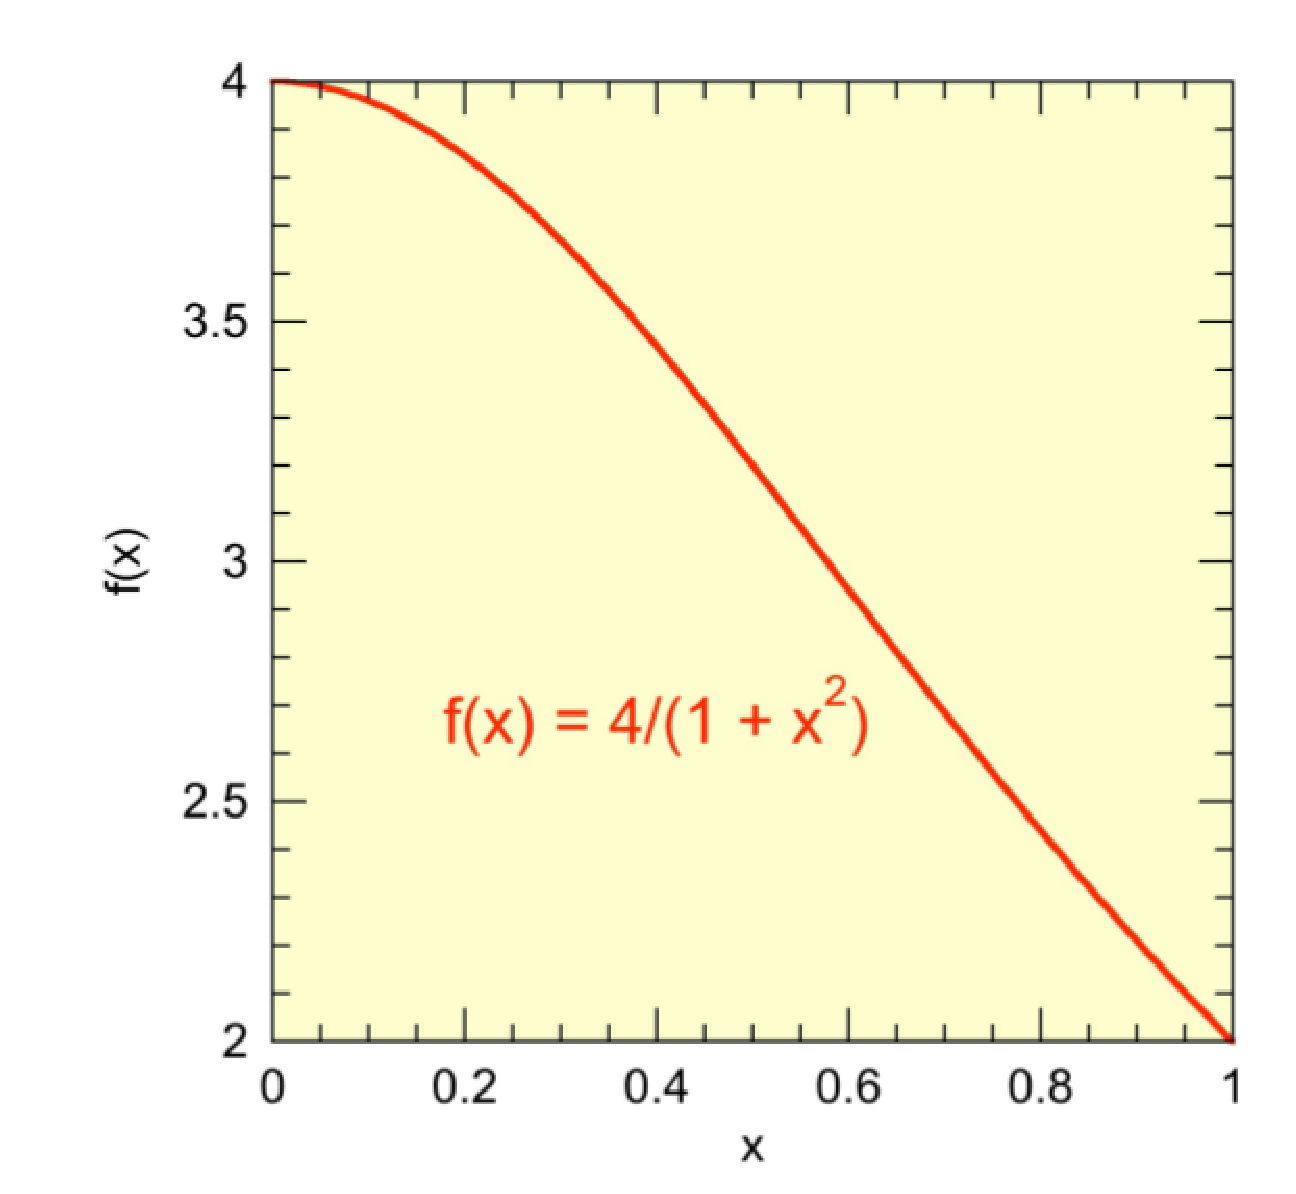
\includegraphics[width=0.6\textwidth]{computepiintegral}
   \caption{微积分形式}\label{fig:computepiintegral}
   \vspace{\baselineskip}
   \end{figure}
    


\section{并行算法}
        
    园周率$\pi$的求解方法具有良好的并行性,可以将任务进行划分,分解为子问题,每个子问题都尅
独立求解计算,
    
    则上述$\pi$的微积分形式离散化表达,见式$1-2$ $$ \sum_{i=0}^{N-1}   \frac{4}{1+x_i^2}\Delta \cong \pi \eqno{{1-2}}$$,其中
    $\Delta = \frac{1}{N}(N=Step)$ , $x_i = (i+0.5)\Delta(i=0,\ldots,N-1)$

   将上述$\pi$的微积分形式离散化,如图~\ref{fig:computepidiscrete}所示  

    \begin{figure}[htbp]
    \centering
    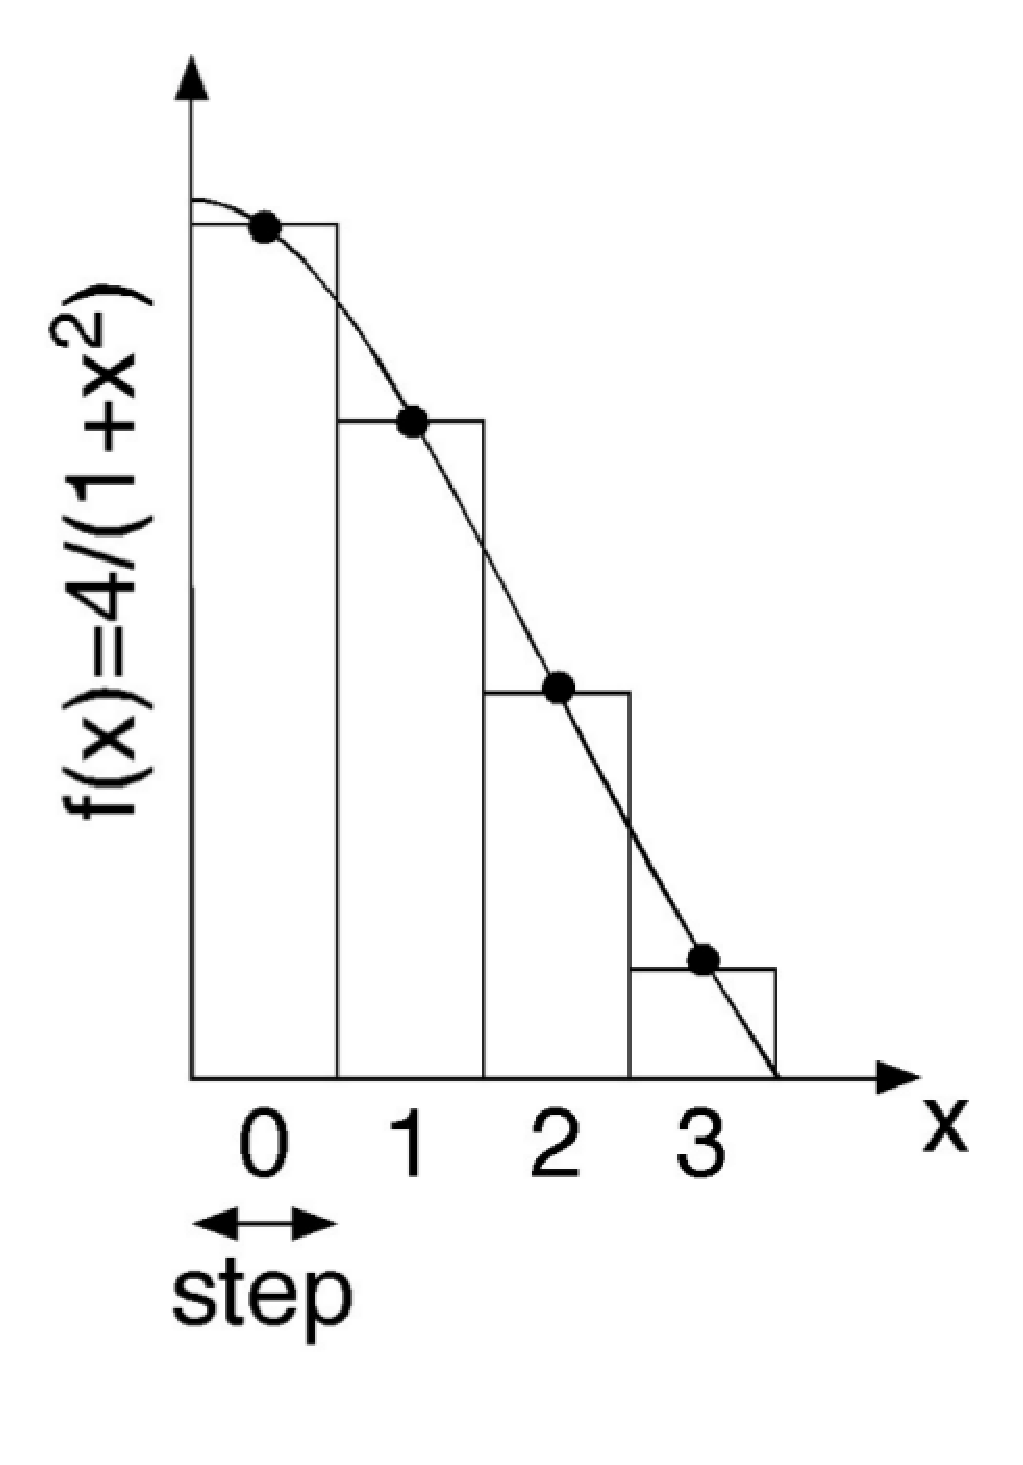
\includegraphics[width=0.6\textwidth]{computepidiscrete}
    \caption{离散化}\label{fig:computepidiscrete}
    \vspace{\baselineskip}
    \end{figure}

    可以将不同Step值读入不同的机器中,广播给各个处理器,每个处理器计算得到自己的结果后,
汇集到主机中.整个算法流程可以表示为图~\ref{fig:pisqe}:
    \begin{figure}[htbp]
    \centering
    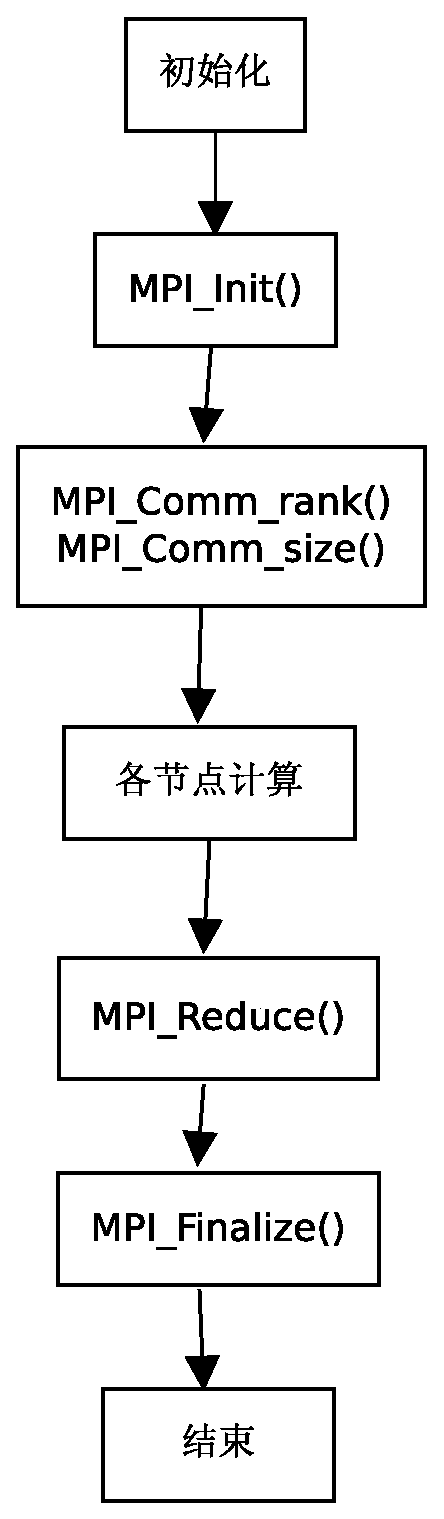
\includegraphics[width=0.3\textwidth]{pisqe}
    \caption{并行化计算$\pi$}\label{fig:pisqe}
    \vspace{\baselineskip}
    \end{figure}


\section{算法伪代码}
    以下部分为算法的伪代码
\algrenewcommand{\algorithmiccomment}[1]{\hskip3em$\rightarrow$ #1}
\begin{algorithmic}[1]
\State $actualpi  \gets 3.141592653589793238462643$
\Comment 初始化真实的$\pi$,对比计算所得的$\pi$
\State $step \gets 1000000;$
\Comment 初始化离散化步数
\State $calcpi,temppi,sum,\ldots$
\State $MPI::Init()$
\Comment 初始化PMI
\State  $intsize \gets  \frac{1}{step} ;partsum \gets  0.1;$
\For{$i \gets  rank+1,n;i+=numproc$}
\Comment $rank 为当前MPI进程的rank值,num_proc为MPI数目$
    \State $    x= intsize *(i-0.5);$
    \State $   partsum += \frac{4}{1+x*x};$
\EndFor
\State $MPI.Reduce(calcpi,partsum);$
\Comment 收集计算所得的pi值
\State $MPI::Finalize()$
\State $总结出来$
\end{algorithmic}

\section{实验结果}
\begin{table}[htbp]
\centering  % 表居中
\begin{tabular}{lcc}  % {lccc} 表示各列元素对齐方式,left-l,right-r,center-c
\hline
Step &非并行算法时间&并行算法时间 \\ \hline  % \hline 在此行下面画一横线
1000&0.001 &0.00014 \\        
10000&0.002 &0.00016 \\      
100000&0.004 &0.00053 \\     
1000000&0.026&0.0081 \\   
10000000&0.187&0.05\\
100000000&1.838 & 0.463\\
1000000000&18.325& 5.46368\\ 
10000000000&15:38.325&7.878 \\ \hline
\end{tabular}
\caption{算法时间对比总结}
\end{table}
%http://www.angio.net/pi/pi-programs.html
%http://www.cnblogs.com/zhangchaoyang/articles/1871168.html
